%%%%%%%%%%%%%%%%%%%%%%%%%%%%%%%%%%%%%%%%%
% Beamer Presentation
% LaTeX Template
% Version 1.0 (10/11/12)
%
% This template has been downloaded from:
% http://www.LaTeXTemplates.com
%
% License:
% CC BY-NC-SA 3.0 (http://creativecommons.org/licenses/by-nc-sa/3.0/)
%
%%%%%%%%%%%%%%%%%%%%%%%%%%%%%%%%%%%%%%%%%

%----------------------------------------------------------------------------------------
%	PACKAGES AND THEMES
%----------------------------------------------------------------------------------------



\documentclass[english]{beamer}

\mode<presentation> {

\usetheme{Madrid}

\definecolor{beamer@udc}{rgb}{0.77, 0, 0.49}
\usecolortheme[RGB={198, 0, 126}]{structure}
\setbeamercolor{alerted text}{fg=beamer@udc}



\setbeamertemplate{navigation symbols}{}
}
\usepackage[english, activeacute]{babel}
\usepackage[utf8]{inputenc} %Codificacion utf-8
\usepackage[official]{eurosym}
\usepackage{verbatim}
\usepackage{fancyvrb}
\usepackage{relsize}
\usepackage[export]{adjustbox}

\usepackage{graphicx} % Allows including images
\usepackage{booktabs} % Allows the use of \toprule, \midrule and \bottomrule in tables


\useinnertheme{circles}
\newenvironment{proenv}{\only{\setbeamercolor{local structure}{fg=green}}}{}
\newenvironment{conenv}{\only{\setbeamercolor{local structure}{fg=red}}}{}


\makeatletter
\setbeamertemplate{footline}
{
  \leavevmode%
  \hbox{%
  \begin{beamercolorbox}[wd=.333333\paperwidth,ht=2.25ex,dp=1ex,center]{author in head/foot}%
    \usebeamerfont{author in head/foot}\insertshortauthor~~(\insertshortinstitute)
  \end{beamercolorbox}%
  \begin{beamercolorbox}[wd=.333333\paperwidth,ht=2.25ex,dp=1ex,center]{title in head/foot}%
    \usebeamerfont{title in head/foot}\insertshorttitle
  \end{beamercolorbox}%
  \begin{beamercolorbox}[wd=.333333\paperwidth,ht=2.25ex,dp=1ex,right]{date in head/foot}%
    \insertframenumber{} / \inserttotalframenumber\hspace*{2ex} 
  \end{beamercolorbox}}%
  \vskip0pt%
}
\makeatother

%----------------------------------------------------------------------------------------
%	TITLE PAGE
%----------------------------------------------------------------------------------------



\title[Harmonization through ASP]{Herramienta para armonización musical\\a través de Answer Set Programming} 

\author[Rodrigo Martín Prieto]{Rodrigo Martín Prieto}
\newcommand{\director}{
\begin{small}
Director:\\José Pedro Cabalar Fernández
\end{small}
}
\institute[UDC] {
Universidade da Coruña \\ % Your institution for the title page
\medskip
\textit{r.martin@udc.es} % Your email address
}
\date{\today} % Date, can be changed to a custom date


\setbeamertemplate{title page}{
\centering
\vfill
\includegraphics[width=0.6\linewidth]{imagenes/anagramaUDC.png}
\vfill
\begin{beamercolorbox}[rounded=true,shadow=true,sep=8pt,center]{title}
\inserttitle \par
\end{beamercolorbox}
Tool for musical harmonization through Answer Set Programming
\vfill
\centering
\insertauthor
\vfill
February 18, 2016\par
\begin{center}
\director
\end{center}

}



\begin{document}

\begin{frame}
\titlepage % Print the title page as the first slide
\end{frame}

%----------------------------------------------------------------------------------------
%	PRESENTATION SLIDES
%----------------------------------------------------------------------------------------

\section{Motivation}
\begin{frame}
	\frametitle{Motivation}
			\begin{beamercolorbox}[leftskip=8cm,center,wd=0.7\textwidth]{author}
			\begin{columns}[T]
			\begin{column}{.60\textwidth}%
				\begin{itemize}
						\item \alert{Musical teaching} is still very traditional nowadays.
						\item Self-teaching of \alert{music theory} is hard.
						\only{
						\item There are not many tools to aid and guide students and self-taught students.
						\item \alert{Composition tools} seek results assuming that the user knows musical theory.
						\item There are intelligent composers: CHASP, Vox Populi, \alert{ANTON}...
						}<2->
				\end{itemize}
			\end{column}
			\begin{column}{.39\textwidth}%
			\includegraphics[width=\linewidth]{imagenes/student-in-class.jpg}
			\end{column}
			\end{columns}
			\end{beamercolorbox}

\end{frame}

\subsection{Background}
\begin{frame}
	\frametitle{Example: Harmonization}
			\begin{beamercolorbox}[leftskip=8cm,center,wd=0.7\textwidth]{author}
			\begin{columns}[T]
			\begin{column}{.60\textwidth}%
\begin{itemize}
		\item \alert{Harmony} is a very important subject in music theory learning
		\item \alert{Choral} music is the root of this subject
		\only{
		\item Exercises consist in \alert{choosing chords sequences} and \alert{completing musical pieces}
		\item Already existing tools do not apply to this particular field
		}<2->
	\end{itemize}
			\end{column}
			\begin{column}{.39\textwidth}%
			\includegraphics[width=\linewidth]{imagenes/tsjsu_choir_02.jpg}
			\end{column}
			\end{columns}
			\end{beamercolorbox}
	
\end{frame}

\subsection{Goals}
	\begin{frame}
		\frametitle{Goals}
			\begin{beamercolorbox}[leftskip=8cm,center,wd=0.7\textwidth]{author}
			\begin{columns}[T]
			\begin{column}{.60\textwidth}%
				\begin{enumerate}
					\item \alert{Harmonize} and annotate chords over any musical score
					\only{\item Given a certain harmonization, be able to complete on purpose \alert{blank sections} of \alert{any incomplete voice} of the score}<2->
					\only{\item \alert{Add new voices} that complement the voices already in the score}<3->
				\end{enumerate}
			\end{column}
			\begin{column}{.39\textwidth}%
			\includegraphics[width=\linewidth]{imagenes/Beethoven.jpg}
			\end{column}
			\end{columns}
			\end{beamercolorbox}
	\end{frame}

\section{Musical Introduction}
\begin{frame}
	\frametitle{Overview}
	\tableofcontents[currentsection,hideothersubsections]
\end{frame}
\subsection{Figures and Rhythm}
	\begin{frame}
		\frametitle{Figures and Rhythm}
		\begin{beamercolorbox}[leftskip=8cm,center,wd=0.7\textwidth]{author}
		\begin{columns}[T]
		\begin{column}{.60\textwidth}%
		\begin{itemize}
			\item Every note is represented by a \alert{figure} that determines it's \alert{length}
			\item Each figure can be \alert{subdivided in two} shorter figures
			\item \alert{Rhythm} is created by \alert{combining figures} of different lengths with special symbols called silences
		\end{itemize}
		\end{column}
		\begin{column}{.39\textwidth}%
		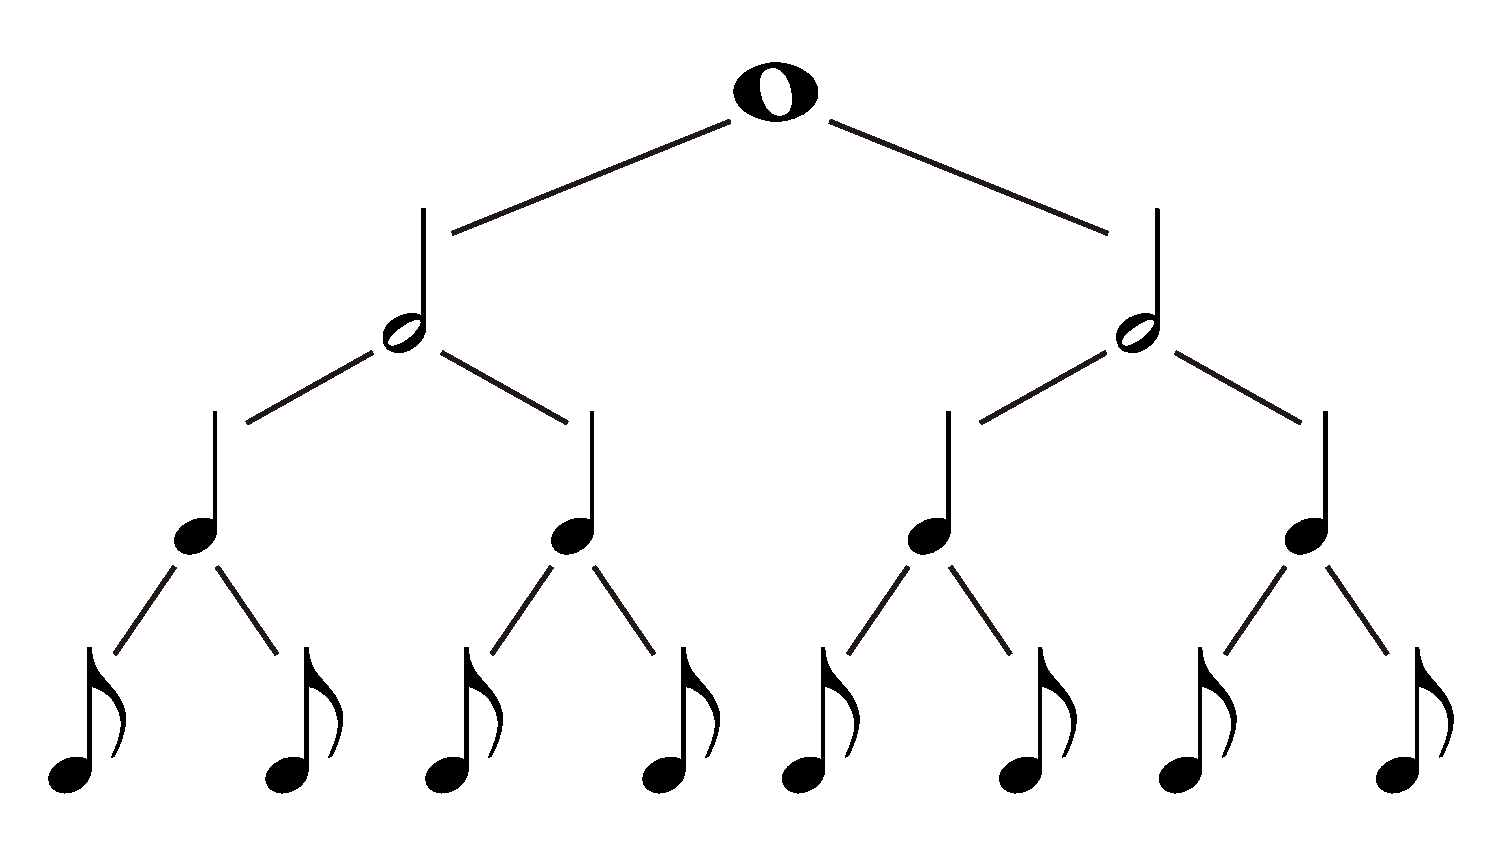
\includegraphics[width=\linewidth]{imagenes/music_tree.pdf}
		\end{column}
		\end{columns}
		\end{beamercolorbox}
		
	\end{frame}
\subsection{Melody}
	\begin{frame}
		\frametitle{Melody}
		\begin{itemize}
			\item \alert{Horizontal} dimension of music
			\item \alert{Pitch} is represented by the \alert{height} at which the note is written, higher position means higher pitch
			\only{
			\item Interval: Jump difference between two notes (including both endpoints)
			}<2->
		\end{itemize}
		\begin{center}
			\only{\includegraphics[width=0.6\linewidth]{imagenes/scores_intervals/C_scale_0-01.png}}<1,2 | handout:0>
			\only{\includegraphics[width=0.6\linewidth]{imagenes/scores_intervals/C_scale_2-01.png}}<3 | handout:0>
			\only{\includegraphics[width=0.6\linewidth]{imagenes/scores_intervals/C_scale_3-01.png}}<4 | handout:0>
			\only{\includegraphics[width=0.6\linewidth]{imagenes/scores_intervals/C_scale_4-01.png}}<5>
			\vfill
			\href{file:///home/trigork/presentation/midi/intro_scale.mp3}{\beamergotobutton{Play}}
		\end{center}
	\end{frame}
\subsection{Tonality}
\begin{frame}
	\frametitle{Tonality}
\end{frame}
\subsection{Harmony}
	\begin{frame}
		\frametitle{Harmony}
		\begin{itemize}
			\item \alert{Vertical} dimension of music
			\item Only present in \alert{polyphonic} pieces or pieces with polyphonic instruments
			\item \alert{Two notes or more} of different voices that play at the same time form a \alert{chord}
			\only{
			\item Fundamental chords of the scale are built adding the third and fifth notes of the root
			}<2->
		\end{itemize}
		\begin{center}
			\only{\includegraphics[width=0.6\linewidth]{imagenes/scores_intervals/C_chords-01.png}}<1,2 | handout:0>
			\only{\includegraphics[width=0.6\linewidth]{imagenes/scores_intervals/C_chords_3-01.png}}<3 | handout:0>
			\only{\includegraphics[width=0.6\linewidth]{imagenes/scores_intervals/C_chords_5-01.png}}<4 | handout:0>
			\only{\includegraphics[width=0.6\linewidth]{imagenes/scores_intervals/C_chords_grades-01.png}}<5>
			\vfill
			\href{file:///home/trigork/presentation/midi/intro_chords.mp3}{\beamergotobutton{Play}}
		\end{center}
		
	\end{frame}

\section{Demo}
\begin{frame}
	\frametitle{Overview}
	\tableofcontents[currentsection,hideothersubsections]
\end{frame}
	\begin{frame}
		\frametitle{Demonstration: Greensleeves}
				\begin{beamercolorbox}[leftskip=8cm,center,wd=0.7\textwidth]{author}
				\begin{columns}[T]
				\begin{column}{.70\textwidth}%
				\includegraphics[width=\linewidth]{imagenes/greensleeves_start.png}
				\end{column}
				\begin{column}{.30\textwidth}%
				 \includegraphics[width=\linewidth]{imagenes/henry_viii.jpg}
				\end{column}
				\end{columns}
				\end{beamercolorbox}
				
	\end{frame}

\section{The Project}
\begin{frame}
	\frametitle{Overview}
	\tableofcontents[currentsection,hideothersubsections]
\end{frame}
\subsection{Architecture}
	\begin{frame}
		\frametitle{haspie's Architecture}
		\begin{figure}
		\centering
		\only{\includegraphics[width=\linewidth]{imagenes/arch_trans/arquitectura_final_asp_nosubs-01.png}}<1 | handout:0>
		\only{\includegraphics[width=\linewidth]{imagenes/arch_trans/arquitectura_final_base-01.png}}<2 | handout:0>
		\only{\includegraphics[width=\linewidth]{imagenes/arch_trans/arquitectura_final_asp_core-01.png}}<3>
				\end{figure}
			\end{frame}
\subsection{ASP Core}
	\begin{frame}[t]
		\frametitle{ASP Core}
		\begin{center}
		\includegraphics[width=0.6\linewidth]{imagenes/arch_trans/arquitectura_final_asp_core-01.png}
		\end{center}
		Answer Set Programming:
		\begin{itemize}
			\item \alert{Independent} of the solving process and its heuristics
			\item The power and \alert{flexibility} of ASP lays on this independence
			\item The problem only needs to be specified by \alert{rules and constraints}
		\end{itemize}
	\end{frame}
	\begin{frame}[fragile]
		\frametitle{ASP Example: the 8 queens problem}
			\begin{Verbatim}[frame=single]
				% Facts
				number(1..8).
				
				% (1) Generate: potential solutions
				1 { q(X,Y) : number(Y) } 1 :- number(X).
				
				% (2) Define: auxiliary predicates
				cell(X,Y) :- number(X), number(Y).
				diff(X,Y,Z,T) :- cell(X,Y), cell(Z,T), X!=Z.
				diff(X,Y,Z,T) :- cell(X,Y), cell(Z,T), Y!=T.
				
				% (3) Test: constraints prune invalid solutions
				:- q(X,Y), q(Z,Y), X!=Z.
				:- q(X,Y), q(X,Z), Y!=Z.
				:- q(X,Y), q(Z,T), diff(X,T,Z,T), |X-Z|=|Y-T|.
			\end{Verbatim}
	\end{frame}
	\begin{frame}[t,fragile]
	\frametitle{Harmonization}
	\begin{center}
			\includegraphics[width=0.6\linewidth]{imagenes/arch_trans/arquitectura_final_asp_harm-01.png}
	\end{center}
	\begin{itemize}
		\item Notes are converted to \alert{grades of the scale} given the \alert{key} and \alert{mode}
		\item \alert{Chords} are assigned to the harmonizable times of the score
		\item \alert{Errors} are computed and the solver determines the \alert{fittest chords} for each section
	\end{itemize}
	\pause
	\begin{Verbatim}[frame=single]
    1 { chord(HT,C) : pos_chord(C) } 1 :- htime(HT).
	\end{Verbatim}
	\begin{center}
			\includegraphics[width=0.25\linewidth,valign=c]{imagenes/example_notes.png}~~
			\includegraphics[width=0.04\linewidth,valign=c]{imagenes/arrow.png}~~
			\includegraphics[width=0.25\linewidth,valign=c]{imagenes/harmonized_example.png}
	\end{center}

	\end{frame}
	\begin{frame}[t,fragile]
	\frametitle{Score Completion}
	\begin{center}
			\includegraphics[width=0.6\linewidth]{imagenes/arch_trans/arquitectura_final_asp_comp-01.png}
			\end{center}
	\begin{itemize}
		\item Only used if there are \alert{new voices or sections} that need to be completed
		\pause
		\item Given the incomplete or new voices' \textit{tessiturae} \alert{notes are assigned} to the available positions
		\pause
		\item \alert{Errors} are computed and solver determines the \alert{fittest notes} for each time
	\end{itemize}
		\begin{center}
				\includegraphics[width=0.25\linewidth,valign=c]{imagenes/incomplete_score.png}~~
				\includegraphics[width=0.04\linewidth,valign=c]{imagenes/arrow.png}~~
				\includegraphics[width=0.25\linewidth,valign=c]{imagenes/completed_score.png}
		\end{center}
	\end{frame}
	\begin{frame}[t,fragile]
	\frametitle{Melodious Preferences Module}
	\begin{center}
			\includegraphics[width=0.6\linewidth]{imagenes/arch_trans/arquitectura_final_asp_pref_mel-01.png}
			\end{center}
	\begin{itemize}
		\item Although not composing melodiously, this module \alert{improves the output in a melodious way}
		\pause
		\item \alert{Checks the tendency} of the voices already on the score and makes the new voices imitate them
		\pause
		\item \alert{Smoothens the melodic jumps} between notes of a same voice
		\item Reduces the number of \alert{consecutive repeated sounds}
	\end{itemize}
		\begin{Verbatim}[frame=single]
		melodic_jump(V,J,B1,B2) :- out_note(V,N1,B1),
		out_note(V,N2,B2),(B1+1) == B2, beat(B1+1), J=|N1-N2|.
		\end{Verbatim}
	\end{frame}
	\begin{frame}[t,fragile]
	\frametitle{Sixths Link Preferences Module}
	\begin{center}
			\includegraphics[width=0.6\linewidth]{imagenes/arch_trans/arquitectura_final_asp_pref_six.png}
			\end{center}
	\begin{itemize}
		\item Progressions of the \alert{second inversion of chords} are very common in choral music
		\item Creates a \alert{per-time harmonization} of the score
		\item \alert{Finds patterns} of second inversion of chords linked in other voices
		\item \alert{Continues and creates} new progressions of this kind if possible
	\end{itemize}
	\begin{Verbatim}[frame=single]
		second_inversion(C,B) :- harmonic_step(V1,V2,4,B), 
		harmonic_step(V1,V3,6,B), beat(B), unary_chord(B,C),V2!=V3.
	\end{Verbatim}
	\end{frame}
	\begin{frame}[fragile]
	\frametitle{User Configuration}
		ASP optimization:
		\begin{itemize}
			\item The \alert{style} of the resulting scores produced by the tool is determined by the optimization of many predicates
			\pause
			\item These optimizations are \alert{weighted} to be able to specify the significance of each of the measured predicates
			\pause
			\item Users can \alert{define their own preferences} by making use of configuration files
		\end{itemize}
		\begin{Verbatim}[frame=single]
			#minimize[out_error(_,_) = chord_errorinstrongw 
                         @ chord_errorinstrongp].
			#minimize[same_chord(_,_) = chord_samechordw
                         @ chord_samechordp].
			#minimize[out_error_weak(_,_) = chord_errorinweakw 
                         @ chord_errorinweakp].
		\end{Verbatim}
	\end{frame}
\subsection{Input}
	\begin{frame}
		\frametitle{haspie's Architecture}
		\begin{center}
		\only{\includegraphics[width=0.95\linewidth]{imagenes/arch_trans/arquitectura_final_asp_core-01.png}}<1 | handout:0>
		\only{\includegraphics[width=0.95\linewidth]{imagenes/arch_trans/arquitectura_final_parser-01.png}}<2>
		\end{center}
	\end{frame}
	\begin{frame}
	\frametitle{Parser and Preprocessor}
		\begin{itemize}
			\item The project also included the development of a lightweight MusicXML parser
			\item Written in \alert{C} with the libraries \alert{Flex and Bison}
			\item Transforms the score in \alert{MusicXML to the ASP logic facts} that the ASP module uses later
			\pause
			\item Performs various tasks as:
				\begin{itemize}
					\item \alert{Subdivides notes} to the length of the smallest figure in the score
					\item Detects most likely key from the score's clef
					\item Reads measure sizes
					\item Transforms \alert{chord names} annotated on score to \alert{grades}
				\end{itemize}
		\end{itemize}
				\begin{center}
						\includegraphics[width=0.25\linewidth,valign=c]{imagenes/example_notes.png}~~
						\includegraphics[width=0.25\linewidth,valign=c]{imagenes/logic_facts_score.png}
				\end{center}
	\end{frame}
\subsection{Output}
	\begin{frame}
		\frametitle{haspie's Architecture}
		\begin{center}
		\only{\includegraphics[width=0.95\linewidth]{imagenes/arch_trans/arquitectura_final_parser-01.png}}<1 | handout:0>
		\only{\includegraphics[width=0.95\linewidth]{imagenes/arch_trans/arquitectura_final_out-01.png}}<2>
		\end{center}
	\end{frame}
		\begin{frame}[t]
		\frametitle{Output Module}
		\begin{center}
				\includegraphics[width=0.6\linewidth]{imagenes/arch_trans/arquitectura_final_out-01.png}
				\end{center}
			\begin{itemize}
				\item Written in \alert{Python} with the toolkit \alert{Music21}
				\item Transforms the internal representation of the solution to a Music21 representation
				\pause
				\item Exports the Music21 representation to the desired format
				\item Some supported formats are Lilypond, PDF, Musescore, MusicXML or MIDI
				\item Allows the result to be \alert{saved or directly shown/played}
			\end{itemize}
		\end{frame}
\subsection{Pipeline}
	\begin{frame}[t]
	\frametitle{Pipeline}
	\begin{center}
			\includegraphics[width=0.6\linewidth]{imagenes/arch_trans/arquitectura_final_pipe-01.png}
			\end{center}
		\begin{itemize}
			\item Written in \alert{Python}
			\pause
			\item Coordinates the different modules secuentially
			\item \alert{Gives feedback} to the user throught the command line
			\pause
			\item Allows the user to pick the desired solution for harmonization and score completion
			\pause
			\item Calls to the \alert{internal representation classes} to store the results of the harmonization and completion as Python objects.
		\end{itemize}
	\end{frame}
\subsection{Methodology and Costs}
\begin{frame}
	\frametitle{Overview}
	    \tableofcontents
	    [currentsection,currentsubsection,hideothersubsections]
\end{frame}
	\begin{frame}
		\frametitle{Custom development cycle}
			\begin{itemize}
			 \item Mix of Spiral and SCRUM
			 \item Each iteration revises previous works and \alert{evolves current prototype}
			 \item Each iteration always has the same phases and these phases are planned beforehand
			 \item The work planned for each iteration is \alert{directed by the objectives}
			 \item Short iterations (1-2 weeks)
			 \item Allows \alert{objective redistribution} for those that can't be achieved in one particular iteration
			 \item Prototypes are revised with the Director after each iteration
			\end{itemize}
	\end{frame}
	\begin{frame}
		\frametitle{Iteration Breakdown and Costs}
		\begin{figure}
		\centering
		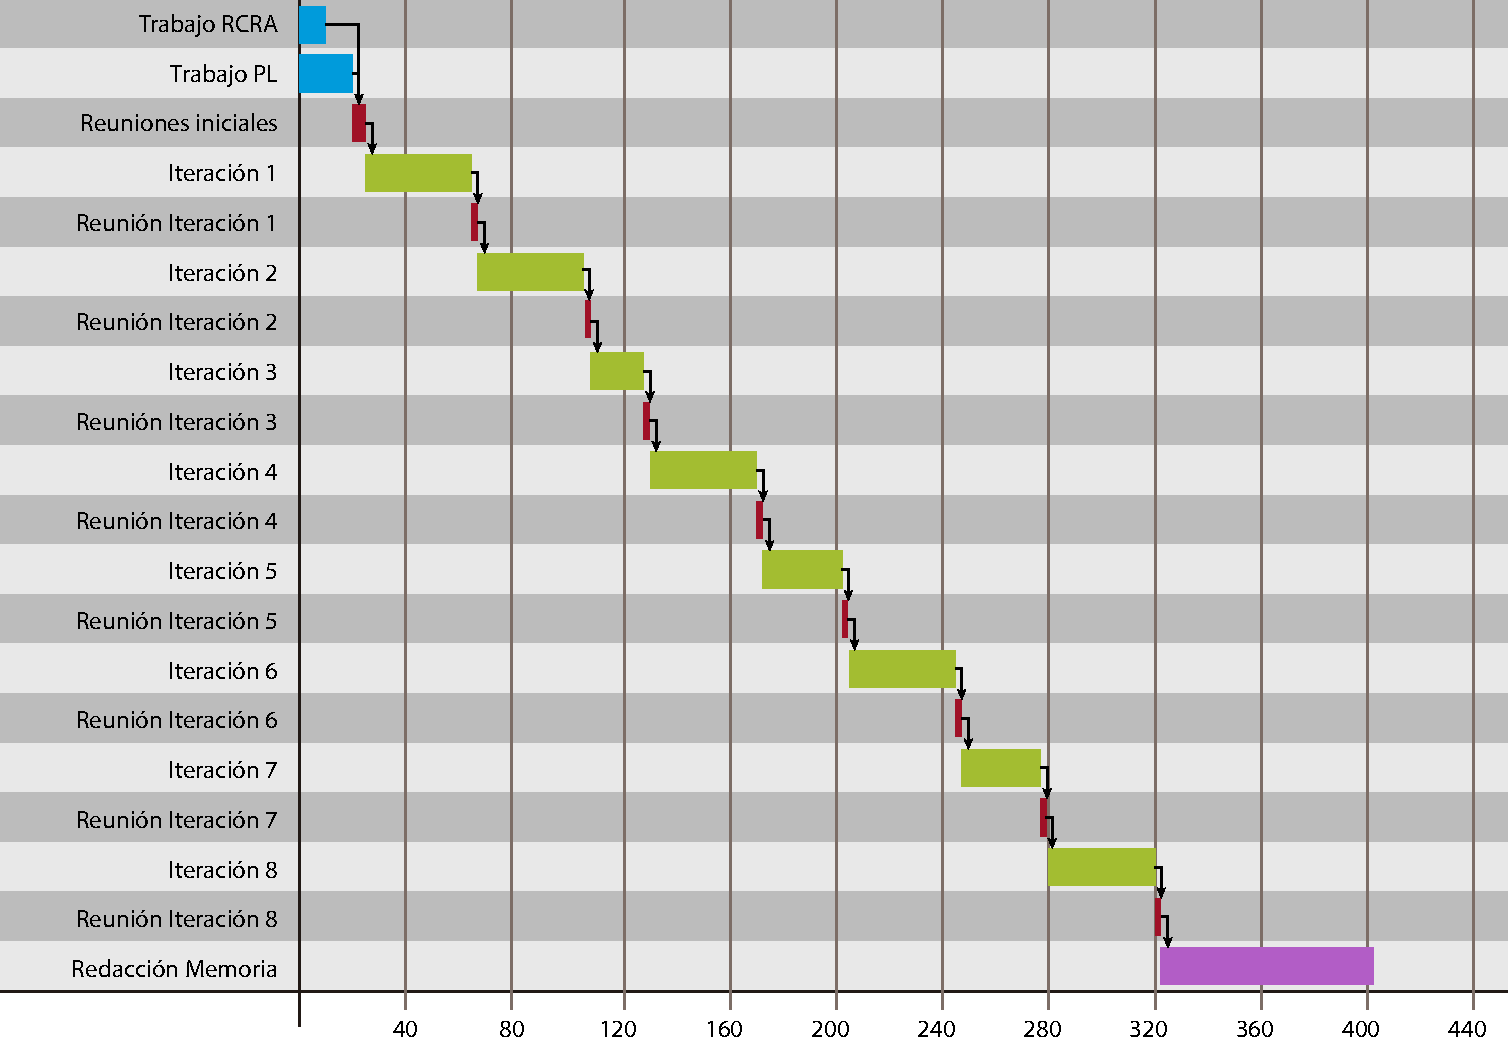
\includegraphics[width=0.7\linewidth]{imagenes/diagrama_tareas.pdf}
		\end{figure}
		
				\begin{table}
				\centering
				\resizebox{0.4\textwidth}{!}{%
					\begin{tabular}{ | l | c | c | c |}
						\hline
						\textbf{Profile} & \textbf{Cost/Hour} & \textbf{Hours} & \textbf{Total} \\ \hline
						Student & 5.5\euro{} & 362 & 1991\euro{} \\ \hline
						Director  & 9\euro{} & 12 & 108\euro{} \\ \hline
						\multicolumn{3}{l}{\textbf{Total}} & 2099\euro{} 
					\end{tabular}}
				\end{table}
	\end{frame}

\section{Conclusions}
\begin{frame}
	\frametitle{Overview}
	\tableofcontents[currentsection,hideothersubsections]
\end{frame}
		\begin{frame}
			\frametitle{Conclusions}
			We developed a system that:
			\begin{enumerate}
				\item \alert{Harmonizes} and annotates chords over almost any score
				\item Given a certain harmonization, \alert{completes blank sections} of the score
				\item \alert{Adds brand new voices} to the score 
			\end{enumerate}
		\end{frame}
		\begin{frame}
			\frametitle{Strengths and Weaknesses}
			\begin{itemize}
				  \item<pro@1-> Achieved \alert{maximum flexibility}
			      \item<pro@1-> The tool produces correct scores in good times
			      \end{itemize}
			      \pause
			      \begin{itemize}
			      \item<con@1-> About 200 ASP lines that are hard to debug
			      \item<con@1-> User still needs \alert{Computer Science and ASP knowledge} to use it
			    \end{itemize}
		\end{frame}
	
\subsection{Future Work}
	\begin{frame}
		\frametitle{Future Work}
		\begin{itemize}
			\item Improve \alert{output} and correct representation mistakes
			\item Implement a \alert{plugin interface} for MuseScore 2 so the tool can be used through the editor itself
			\item Research about \alert{modulation} and implement it in the tool
			\item Improve execution times for the inclusion of new voices
			\item Include \alert{rhythmic patterning} in the new generated voices
			\item Ask for feedback from professional harmony teachers and polish the tool so it can be used in teaching
		\end{itemize}
	\end{frame}
		
\begin{frame}
\centering
\vfill
\includegraphics[width=0.6\linewidth]{imagenes/anagramaUDC.png}
\vfill
\begin{beamercolorbox}[rounded=true,shadow=true,sep=8pt,center]{title}
\inserttitle \par
\end{beamercolorbox}
\vfill
\centering
\insertauthor
\vfill
February 18, 2016\par
\begin{center}
\director \par 
\vfill
\alert{Thank you!}
\end{center}
\end{frame}


\end{document} 